%%%%%%%%%%%%%%%%%%%%%%%%%%%%%%%%%%%%%%%%%%%%%%%%%%%%%%%%%%%%%%%%%%%%%%%%%%%%%%%%%%%%%%%%%%%%%%%%%%%%%%
%
%   Filename    : appendix_B.tex
%
%   Description : This file will contain information about your Resource Persons
%                 
%%%%%%%%%%%%%%%%%%%%%%%%%%%%%%%%%%%%%%%%%%%%%%%%%%%%%%%%%%%%%%%%%%%%%%%%%%%%%%%%%%%%%%%%%%%%%%%%%%%%%%

\chapter{Supplementary Analysis}
\label{sec:appendixb}

%
%  Indicate your resource persons here:
%
%	<full name and title, e.g., Dr. Juan de la Cruz>
%	<profession, e.g., faculty>
%	<department, e.g., Division of Physical Sciences and Mathematics>
%	<name of institution, e.g., University of the Philippines Visayas>
%	<e-mail address>
%
%

\begin{figure}[!htbp]
	\centering
	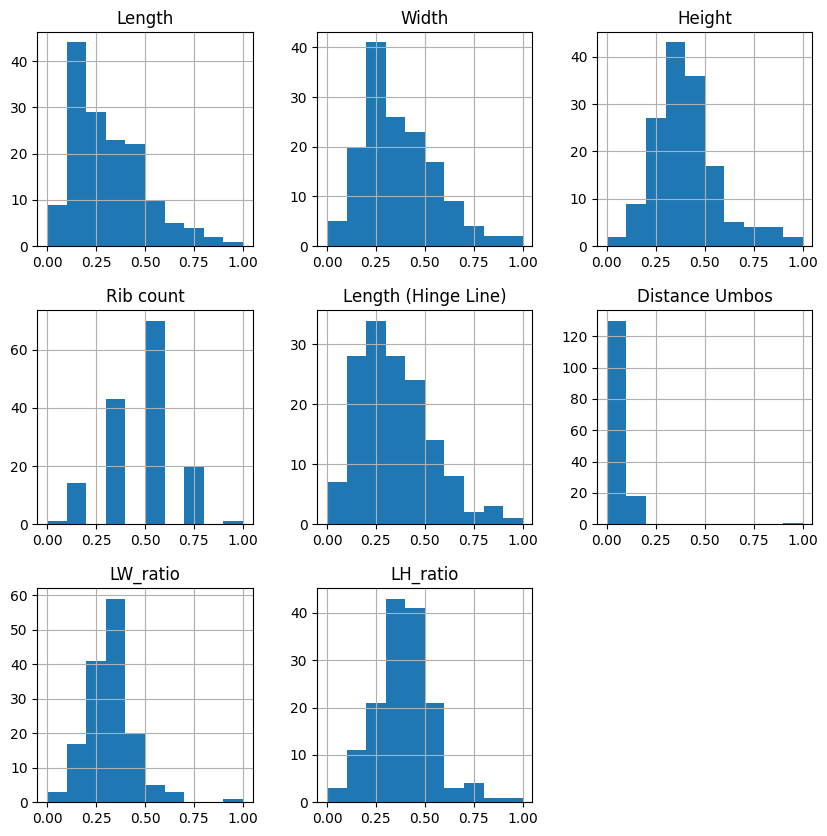
\includegraphics[width=0.6\textwidth]{figures/sample_distribution.png}
	\caption{Feature Distribution of \Tegillarcagranosa}
\end{figure}

\begin{figure}[!htbp]
	\centering
	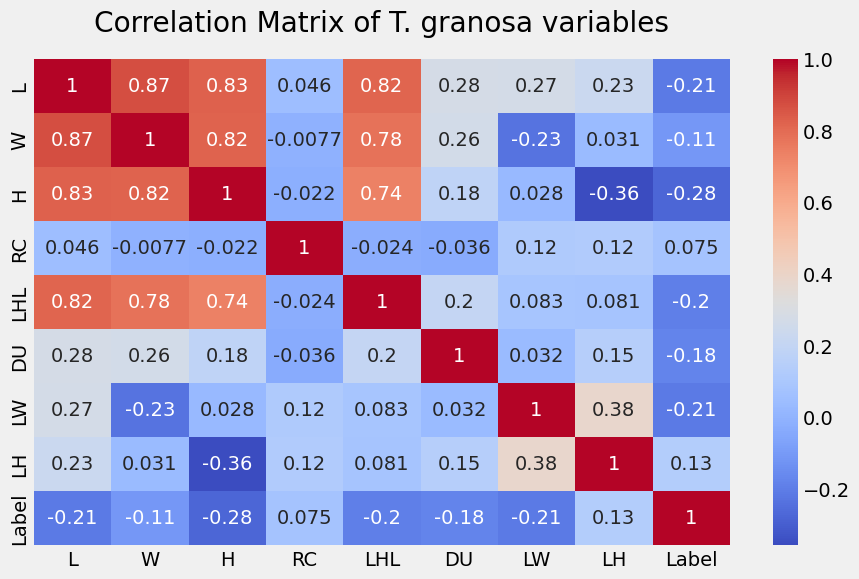
\includegraphics[width=0.8\textwidth]{figures/corr_matrix.png}
	\caption{Correlation Matrix of Morphological Variables \Tegillarcagranosa}
\end{figure}

\begin{figure}[!htbp]
	\centering
	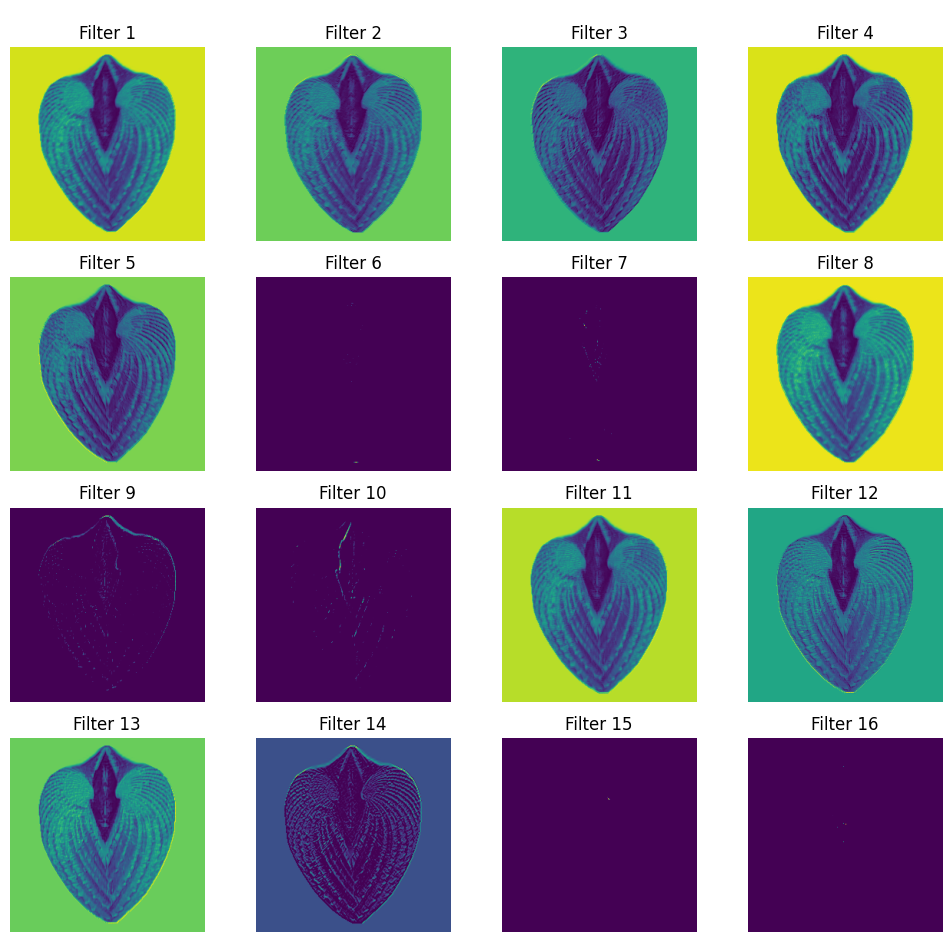
\includegraphics[width=0.6\textwidth]{figures/conv1.png}
	\caption{Feature Maps from First Convolution Layer}
\end{figure}

\begin{figure}[!htbp]
	\centering
	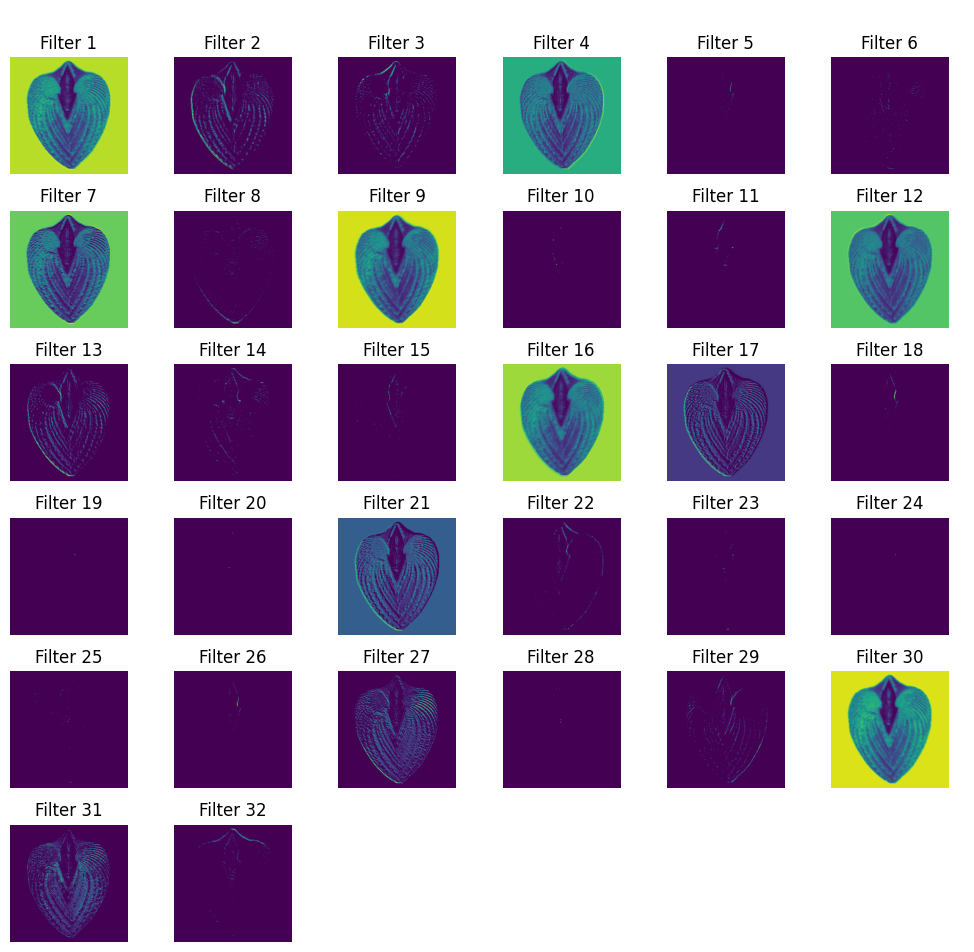
\includegraphics[width=0.6\textwidth]{figures/conv2.png}
	\caption{Feature Maps from Second Convolution Layer}
\end{figure}

\begin{figure}[!htbp]
	\centering
	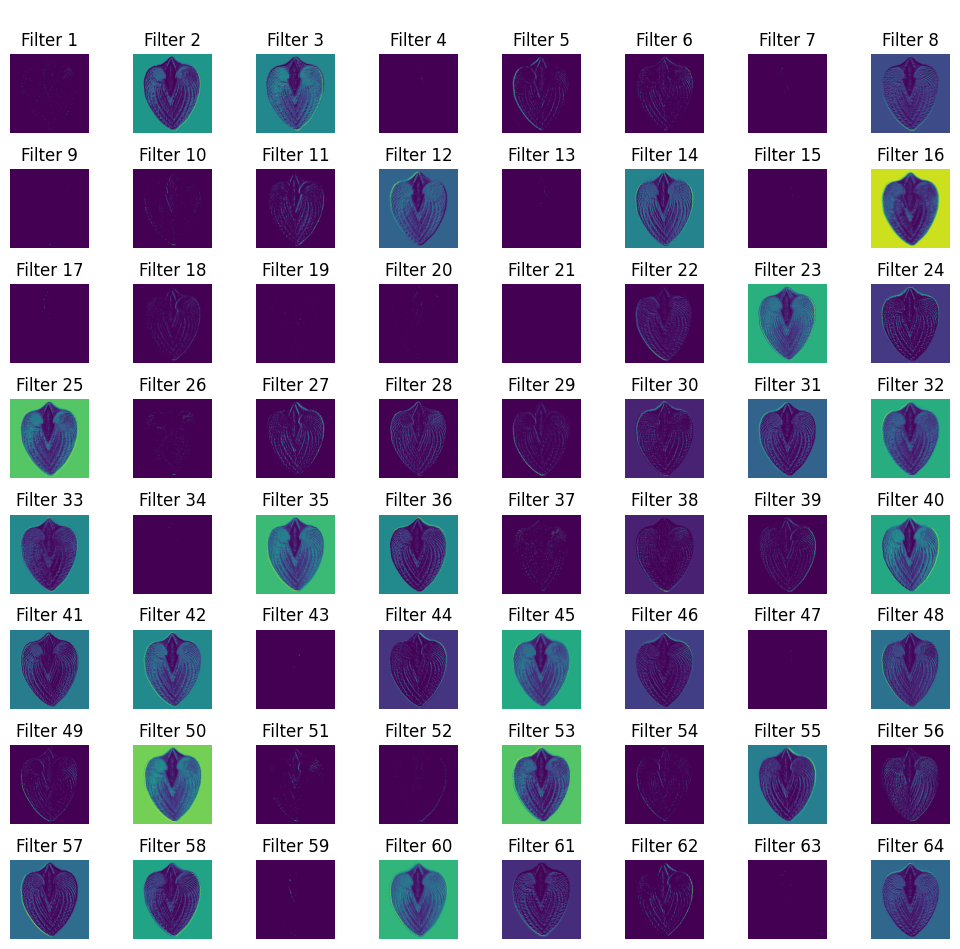
\includegraphics[width=0.6\textwidth]{figures/conv3.png}
	\caption{Feature Maps from Third Convolution Layer}
\end{figure}